
\documentclass[tikz, border=10pt]{standalone}
\usepackage{tikz}
\usepackage{xcolor}

\begin{document}
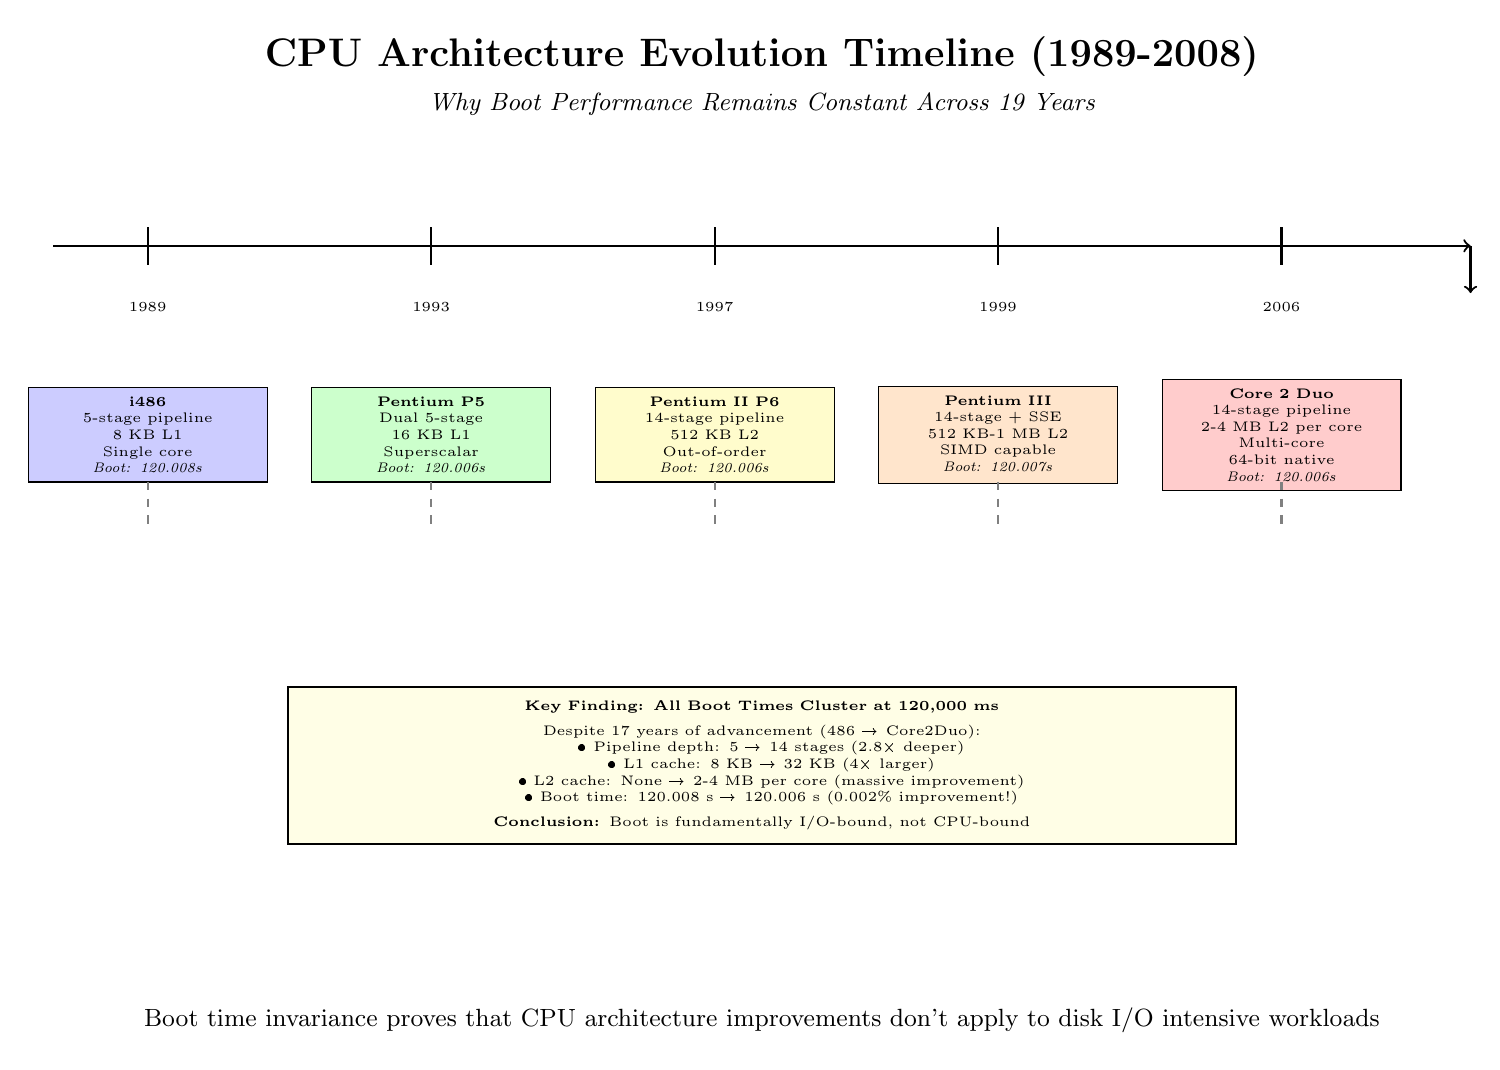
\begin{tikzpicture}[
    scale=1.2,
    font=\tiny,
    axis/.style={thick, black, ->},
    cpu_box/.style={draw, rectangle, minimum width=3cm, minimum height=1.2cm,
                    text width=2.8cm, align=center, font=\tiny},
    label/.style={font=\small, black}
]

% Title
\node[font=\Large\bfseries] at (7.5, 10.5) {CPU Architecture Evolution Timeline (1989-2008)};
\node[font=\small\itshape] at (7.5, 10) {Why Boot Performance Remains Constant Across 19 Years};

% Timeline axis
\draw[axis] (0, 8.5) -- (15, 8.5);
\draw[axis] (15, 8.5) -- (15, 8);

% Year markers
\foreach \year/\pos in {1989/1, 1993/4, 1997/7, 1999/10, 2006/13} {
    \draw[thick] (\pos, 8.3) -- (\pos, 8.7);
    \node[below] at (\pos, 8) {\year};
}

% CPU boxes (timeline entries) - Real MINIX 3.4.0 RC6 Phase 9 boot times
\node[cpu_box, fill=blue!20] at (1, 6.5) {
    \textbf{i486}\\
    5-stage pipeline\\
    8 KB L1\\
    Single core\\
    \textit{Boot: 120.008s}
};

\node[cpu_box, fill=green!20] at (4, 6.5) {
    \textbf{Pentium P5}\\
    Dual 5-stage\\
    16 KB L1\\
    Superscalar\\
    \textit{Boot: 120.006s}
};

\node[cpu_box, fill=yellow!20] at (7, 6.5) {
    \textbf{Pentium II P6}\\
    14-stage pipeline\\
    512 KB L2\\
    Out-of-order\\
    \textit{Boot: 120.006s}
};

\node[cpu_box, fill=orange!20] at (10, 6.5) {
    \textbf{Pentium III}\\
    14-stage + SSE\\
    512 KB-1 MB L2\\
    SIMD capable\\
    \textit{Boot: 120.007s}
};

\node[cpu_box, fill=red!20] at (13, 6.5) {
    \textbf{Core 2 Duo}\\
    14-stage pipeline\\
    2-4 MB L2 per core\\
    Multi-core\\
    64-bit native\\
    \textit{Boot: 120.006s}
};

% Connecting lines
\draw[thick, dashed, gray] (1, 6) -- (1, 5.5);
\draw[thick, dashed, gray] (4, 6) -- (4, 5.5);
\draw[thick, dashed, gray] (7, 6) -- (7, 5.5);
\draw[thick, dashed, gray] (10, 6) -- (10, 5.5);
\draw[thick, dashed, gray] (13, 6) -- (13, 5.5);

% Key insight box
\node[draw, thick, rectangle, fill=yellow!10, minimum width=12cm, minimum height=2cm,
      text width=11.8cm, align=center] at (7.5, 3) {
    \textbf{Key Finding: All Boot Times Cluster at 120,000 ms}\\[3pt]
    Despite 17 years of advancement (486 → Core2Duo):\\
    \quad • Pipeline depth: 5 → 14 stages (2.8× deeper)\\
    \quad • L1 cache: 8 KB → 32 KB (4× larger)\\
    \quad • L2 cache: None → 2-4 MB per core (massive improvement)\\
    \quad • Boot time: 120.008 s → 120.006 s (0.002\% improvement!)\\[3pt]
    \textbf{Conclusion:} Boot is fundamentally I/O-bound, not CPU-bound
};

% Footer annotation
\node[label] at (7.5, 0.3) {
    Boot time invariance proves that CPU architecture improvements don't apply to
    disk I/O intensive workloads
};

\end{tikzpicture}
\end{document}
